\chapter{Experiments} \label{experiments}
In this chapter, we will carry out some experiments to test the improvements made in chapters \ref{IDPL} and \ref{IEBT}.
For the execution of the programs, I will be using an Asus VivoBook 15 X540UB laptop. These are the technical specifications of the laptop:
\begin{itemize}
  \item \textbf{Processor:}  Intel Core i5-8250U CPU @ 1.60GHz
  \item \textbf{Memory}  8GB RAM
  \item \textbf{Graphics adapter:} Intel UHD Graphics 620
  \item \textbf{Storage:} 256 SSD
  \item \textbf{Operating System:} Windows 10 Home 64-bit
\end{itemize}
To ensure better results, they will all be executed with the laptop running only that process.
In all experiments, only the execution time will be evaluated.
Memory usage would remain to be checked to complete the evaluation.\\
All the experiments and results can be found in the 'Experiments' folder on Github. \cite{forner_gomez_source_nodate}

\section{Testing Library}
The main improvement that can affect the performance of the library is the update of GHC.
To test this, we will use the toy problem developed during this work.
We will modify it a bit by counting characters instead of words, in order to be able to test larger inputs more efficiently.
We will limit the characters to those of the alphabet (plus the dot for the incremental character) thus ensuring that there will be at most 26 filters.
\subsection*{Input}
The text of Don Quixote has been used as input, which has been modified to convert or eliminate any unwanted characters.
To do this function, a python script has been used that also allows generating inputs of a specific size.
Inputs of powers of 10 will be used, from 10 to 100000.

\subsection*{Results}
These are the results of running 10 times for each size and taking the mean and standard deviation.

\begin{table}[H]
    \begin{adjustwidth}{-1in}{-1in} % Adjust margins by -1 inch on both sides
    \centering
    \begin{tabular}{|c|c|c|c|c|c|c|c|c|c|c|c|c|}
    \hline
    size & mean (s)& std (s) \\
    \hline
    10 & 0.029994 & 0.012285 \\
    100 & 0.100318 & 0.008902 \\
    1000 & 0.971935 & 0.097618 \\
    10000 & 11.619426 & 0.835211 \\
    100000 & 231.629199 & 1.330213 \\
    \hline
    \end{tabular}
    \caption[{[Exp] Table results GHC 8.10.3}]{Results 10 executions using GHC 8.10.3}
    \label{results1}
    \end{adjustwidth}
\end{table}

\begin{table}[H]
    \begin{adjustwidth}{-1in}{-1in} % Adjust margins by -1 inch on both sides
    \centering
    \begin{tabular}{|c|c|c|c|c|c|c|c|c|c|c|c|c|}
    \hline
    size & mean (s)& std (s) \\
    \hline
    10 & 0.005374 & 0.001071 \\
    100 & 0.091677 & 0.004923 \\
    1000 & 0.881183 & 0.067268 \\
    10000 & 9.786606 & 0.606498 \\
    100000 & 159.005325 & 1.553883 \\
    \hline
    \end{tabular}
    \caption[{[Exp] Table results GHC 9.0.2}]{Results 10 executions using GHC 9.0.2}
    \label{results2}
    \end{adjustwidth}
\end{table}

\begin{figure}[H]
    \centering
    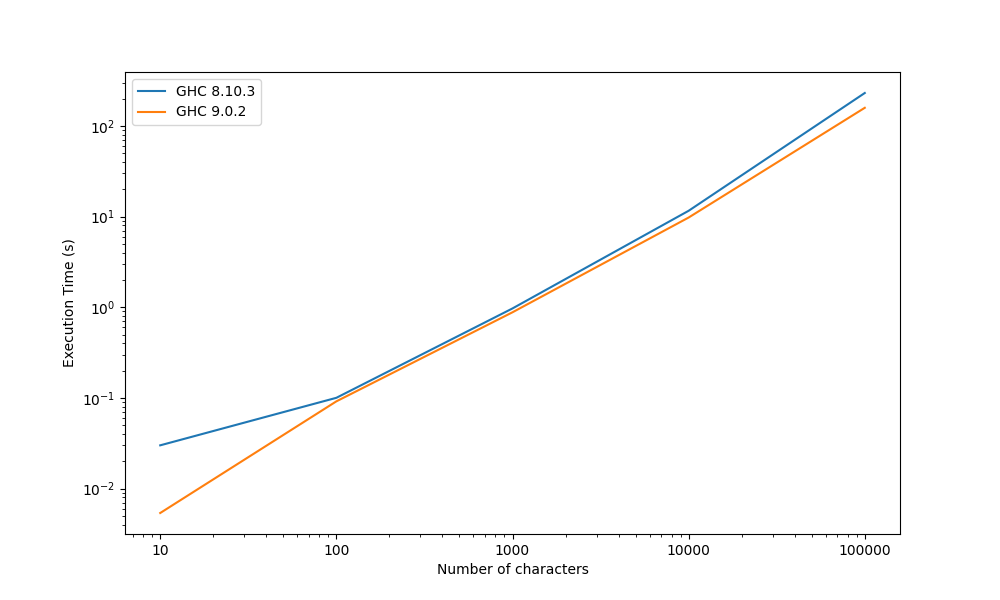
\includegraphics[width=1\textwidth]{ExecutionPlot.png}
    \caption[{[Exp] Plot GHC 8.10.3 vs 9.0.2}]{Plot of execution mean time vs input size for GHC 8.10.3 and GHC 9.0.2}
    \label{fig:results3}
\end{figure}

\subsection*{Discussion}
As we can observe, there seems to be a slight improvement with GHC 9.02 compared to GHC 8.10.3, even in some more noticeable cases. \\

We can see how for much smaller inputs the new version tends to obtain better results, which could be due to better management when creating the filters.
In smaller inputs, the task that is done the most is generating filters, because with larger inputs there comes a point where the 26 filters have already been generated (one for each letter) and no more are generated.
Perhaps better memory management by the compiler is causing this improvement. \\
On the other hand, we can observe how in the central part the two have a similar performance, although the new version is still slightly better. \\
Finally, we can see how with larger inputs the new version again has better performance, this time more noticeable. \\

In summary, although it seems that with the update to GHC 9.0.2 there is an improvement, we do not obtain very clear results.
Other factors such as memory would have to be checked to conclude with a result.

\section{Testing IEBT}
In this experiment, we will test the change of structure from Set to HashSet implemented in the IEBT algorithm.

\subsection*{Input}
For this experiment, we will be using a bipartite graph of 3000 edges and we will make queries from size 1000 edges to 3000.

\subsection*{Results}
This is the result of running each size 5 times and obtaining the mean and standard deviation.

\begin{table}[H]
    \begin{adjustwidth}{-1in}{-1in}
    \centering
    \begin{tabular}{|c|c|c|c|c|c|c|c|c|c|c|c|c|}
    \hline
    size & mean (s)& std (s) \\
    \hline
    1000 & 5.570314 & 0.560374 \\
    1500 & 7.731554 & 1.032222 \\
    2000 & 8.778615 & 1.534666 \\
    2500 & 9.506494 & 0.579319 \\
    3000 & 12.134800 & 2.795664 \\
    \hline
    \end{tabular}
    \caption[{[Exp] Table results Set structure}]{Results 5 executions using Set structure}
    \label{results4}
    \end{adjustwidth}
\end{table}

\begin{table}[H]
    \begin{adjustwidth}{-1in}{-1in} % Adjust margins by -1 inch on both sides
    \centering
    \begin{tabular}{|c|c|c|c|c|c|c|c|c|c|c|c|c|}
    \hline
    size & mean (s)& std (s) \\
    \hline
    1000 & 7.677365 & 0.378990 \\
    1500 & 8.242099 & 1.010196 \\
    2000 & 8.417874 & 0.367513 \\
    2500 & 9.013060 & 0.483033 \\
    3000 & 9.586805 & 1.195353 \\
    \hline
    \end{tabular}
    \caption[{[Exp] Table results HashSet structure}]{Results 5 executions using HashSet structure}
    \label{results5}
    \end{adjustwidth}
\end{table}

\begin{figure}[H]
    \centering
    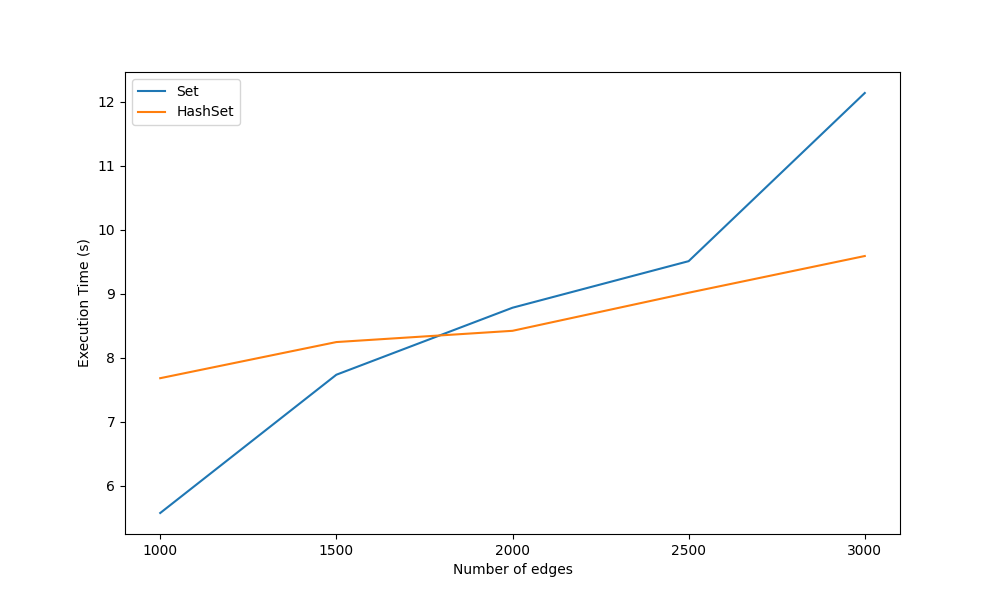
\includegraphics[width=1\textwidth]{ExecutionPlot2.png}
    \caption[{[Exp] Plot Set vs HashSet}]{Plot of execution mean time vs input size for Set and HashSet}
    \label{fig:results6}
\end{figure}

\subsection*{Discussion}
We can see that it seems that we have obtained a performance improvement when the input starts to grow.\\
For smaller inputs, Set obtains better performance, surely because the overhead of making HashSet calculations is high and Set has better performance.
On the other hand, when the input grows, we see how HashSet remains more stable and grows in a more linear way, while Set grows faster due to the overhead of doing the searches.\\

In short, we can conclude that this change has been positive, although it is only for large input types of edges, not for the general case of the algorithm.